\section{Simplex Category and Simplicial Sets}

\subsection{Simplex Category}

The goal of this mini-project to to define $\infty$-categories via simplicial sets. 
The definition of simplicial sets is based on the \emph{simplex category}, $\D$.

\begin{definition}[Simplex Category \cite{lurie}]
	The \emph{simplex category}, denoted as $\D$, is the category of ordinal numbers. 
	Precisely
	\begin{enumerate}
		\item Its objects are linearly ordered finite sets $[n] = \{0 < 1 < \cdots < n\}$ for all $n \geq 0$.
	\item Morphisms are given by order-preserving maps.
	\end{enumerate}
	Simplex category is also known as the category of combinatorial simplices
\end{definition}

It is clear that $\D$ is equivalent to the category of all finite non-empty totally ordered sets with order-preserving maps. 

For each $n, j \in \N, 0\leq j \leq n$, define a sequence of \emph{face} and \emph{degenerate} maps with repective notations as $d^{j,n}: [n - 1] \to [n]$ and $s^{j, n}: [n + 1] \to [n]$, 
\begin{equation}
	d^{j, n}(i) = \begin{cases}
		i & i < j \\
		i + 1 & i \geq j
	\end{cases}, \quad
	s^{j,n}(i) = \begin{cases}
		i & i \leq j \\
		i - 1 & i > j
	\end{cases}.
\end{equation}

Concretely, the face map $d^{j, n}$ is the only injective and order-preserving maps from $[n - 1]$ to $[n]$ that misses $j \in [n]$, and the degenerate map $s^{j, n}$ is the only surjective and order-preserving map from $[n + 1]$ to $[n]$ that hits $j \in [n]$ twice.

Since the domain and codomain of the face and degenerate maps will always be clear from the context, we will drop the superscripts and denote them as $d^j$ and $s^j$.

Let $i < j$. 
The composition of face maps $d^jd^i$ is the unique injective and order-preserving map from $[n - 2]$ to $[n]$ that misses both $i$ and $j \in [n]$. 
A moment of thought shows that this map is the same as $d^id^{j - 1}$.
There are similar relations for the compositions of degenerate maps and mixed compositions of face and degenerate maps. 
All of the identities are listed below.

% TODO: check the middle case
\begin{align}
	d^jd^i &= d^id^{j - 1}, \quad i < j \label{sim1} \\
	s^js^i &= s^is^{j + 1}, \quad i \leq j  \label{sim2} \\
	s^j d^i &= \begin{cases}
		d^i s^{j - 1} & j < i \\
		\text{id} & j = i, i + 1 \\
		d^{i - 1} s^j & j > i + 1
	\end{cases} \label{sim3}
\end{align}

Let me introduce a temporary notation for order-preserving maps in $\D$.
Denote an order-preserving map $\alpha: [m] \to [n]$ as a sequence $[a_0, a_1, \cdots, a_m]$, which means where $a_i = \alpha(i)$.
For example the face map $d^0 : [2] \rightarrow [3]$ can be denoted as $[1, 2, 3]$, and the degenerate map $s^1: [3] \to [2]$ can be denoted as $[0, 1, 1, 2]$.

For any order-preserving map $\alpha: [m] \to [n]$, it must have the form 
$$
[\underbrace{\alpha_0, \cdots, \alpha_0}_{c_0}, \underbrace{\alpha_1, \cdots, \alpha_1}_{c_1}, \cdots, \underbrace{\alpha_k, \cdots, \alpha_{k-1}}_{c_{k-1}}]
$$
where $\alpha_i \in [n]$, $\alpha_i < \alpha_j$ if $i < j$ and $\sum c_i = m+1$.
This notation means precisely that $\alpha$ sends the first $c_0$ elements of $[m]$ to $\alpha_0$, the next $c_1$ elements to $\alpha_1$, and so on.

Consider the surjective map $\eta': [m] \rightarrow [k]$ defined as 
$$
[\underbrace{0, \cdots, 0}_{c_0}, \underbrace{1, \cdots, 1}_{c_0}, \cdots, \underbrace{k - 1, \cdots, k - 1}_{c_{k-1}}] 
$$
Notice that $\eta'$ can be written as a composition of degenerate maps
$$
\eta' = \underbrace{s^{m - c_k} \cdots s^{m - c_k}}_{c_{k - 1} - 1} \cdots \underbrace{s^{c_1} \cdots s^{c_1}}_{c_1 - 1} \underbrace{s^0 \cdots s^0}_{c_0 - 1}.
$$

Consider the injective map $\epsilon': [k] \rightarrow [n]$ defined as 
$$
[\alpha_0, \alpha_1, \cdots, \alpha_{k-1}].
$$
Similarly, $\epsilon'$ can be written as a composition of face maps
$$
\epsilon' = \underbrace{d^0 \cdots d^0}_{\alpha_0} \underbrace{d^{\alpha_0 + 1} \cdots d^{\alpha_0 + 1}}_{\alpha_1 - \alpha_0 - 1} \cdots \underbrace{d^{\alpha_{k-1} + 1} \cdots d^{\alpha_{k-1} + 1}}_{ \alpha_{k-1} - \alpha_{k-2} - 1}.
$$
It is clear that $\alpha = \epsilon' \eta'$. 
Therefore, we have proved the following two theorems.
\begin{lemma}
	Every morphism in the simplex category $\D$ can be written as a composition of face and degenerate maps.
\end{lemma} 

\begin{lemma}\label{epi-mono-simplex}
	Every morphism $\alpha: [m] \to [n]$ in the simplex category $\D$ has a unique epi-mono factorisation $\alpha = \epsilon \eta$ where $\eta: [m] \to [k]$ is a composition of degenerate maps and $\epsilon: [k] \to [n]$ is a composition of face maps.
\end{lemma}

We are now ready to define simplicial sets.

\subsection{Definition of Simplicial Set}


\begin{definition}[Simplicial Set \cite{lurie}]
	A \emph{simplicial set} is presheaf on $\D$, i.e.,
	a functor $X: \D\op \to \S$. 
	We will denote the category of simplicial sets as $\sS$.
\end{definition}

Let $X$ be a simplicial set.
Denote $X_n := X([n])$.
We shall define the face map $d_j: X_n \rightarrow X_{n-1}$ as the map induced by the face map on $\D$, $d^j: [n - 1] \to [n]$. 
That is $d_j = Xd^j$. 
Similarly, denote $s_j: X_n \to X_{n + 1}$ the map induced by the degenerate map $s^j: [n + 1] \to [n]$, i.e., $s_j = Xs^j$.
Since $X$ is contravariant, $d_j$ and $s_j$ will satify the following identities, reversing the order of composition compared to \eqref{sim1}, \eqref{sim2}, and \eqref{sim3}. 
\begin{align}
	d_i d_j &= d_{j - 1} d_i, \quad i < j \label{simp1} \\
	d_i s_j &= \begin{cases}
		s_{j - 1} d_{i} & j < i \\
		\text{id} & j = i, i + 1 \\
		s_{j} d_{i - 1} & j > i + 1
	\end{cases} \label{simp3} \\
	s_i s_j &= s_{j + 1} s_i, \quad i \leq j  \label{simp2} 
\end{align}

Since $d^j$ and $s^j$ generates all morphisms in $\D$, the morphisms $d_j$ and $s_j$ will generate all relevant morphisms in $\S$ relevant to $X$ (Recall $X \in [\D\op, \S]$). 
This gives a crucial observation. 

\begin{remark}\label{rm:sim-set-data}
The data given by a simplicial set $X$ is equivalent to the data of a sequence of sets $\{X_n\}_{n \geq 0}$ together with face and degenerate maps $d_j: X_n \to X_{n - 1}$ and $s_j: X_n \to X_{n + 1}$ satisfying the identities \eqref{simp1}, \eqref{simp2}, and \eqref{simp3}.
\end{remark}

An element in $X_n$ is called an \emph{n-simplex} of $X$. 
It is \emph{degenerate} if it is in the image of some degenerate map $s_j: X_{n - 1} \to X_n$ for some $0 \leq j \leq n - 1$, and \emph{non-degenerate} otherwise.

The first intuitive example of simplicial sets are the standard simplices, which are the Yoneda embeddings of the objects in $\D$.

\begin{definition}[Standard n-Simplex \cite{lurie}]
	For each $n \geq 0$, the \emph{standard n-simplex}, denoted as $\Delta^n$, is defined as the contravairant functor
	\begin{equation*}
		\Delta^n := \H_{\D}(-, [n]): \D\op \to \S.
	\end{equation*}
\end{definition}

\begin{remark}
	By the Yoneda lemma, for any simplicial set $X$, there is a natural isomorphism
\begin{equation*}
	\H_{\sS}(\Delta^n, X) \cong X_n.
\end{equation*}
\end{remark}

\begin{example}
	\begin{enumerate}
		\item For each $m \geq 0$, there is a unique map from $[m]$ to $[0]$ in $\D$, and $\Delta^0([m])$ is a singleton set for all $m \geq 0$, with a unique morphism between any $\Delta^0[m]$ and $\Delta^0[k]$. Therefore $\Delta^0$ is the \textit{terminal object} in $\sS$ following remark \ref{rm:sim-set-data}. Given any simplicial set $X$, the unique morphism from $X$ to $\Delta^0$ sends all element of $X_n$ is sent to the unique element of $\Delta^0[n]$. This obviously satifies the naturality condition, as there is only one morphism in $\Delta^0$ between any simplices.
		\item The initial object in $\sS$ is the empty set.
		\item In $\Delta^n$, the unique non-degenerate element is the identity map $\text{id}_{[n]} \in \Delta^n[n]$.
			All other elements in $\Delta^n[m]$ for $m \neq n$ are degenerate.
	\end{enumerate}
\end{example}

Another important class of simplicial sets are horns, which can be thought of as subsets of standard simplices.

\begin{definition}[Horn \cite{lurie}]
	For each $n \geq 1$ and $0 \leq i \leq n$, the \emph{$i$-th horn}, denoted as $\L^n_i$, is the simplicial defined as
	\begin{enumerate}
		\item $\L^n_i([m]) = \{f \in \H_{\D}([m], [n]) : [n] \smallsetminus \{i\} \not\subseteq f([m])\}$. 
			In other words, $\L^n_i ([m])$ is the set of all order-preserving maps from $[m]$ to $[n]$ that miss at least one element in $[n] \smallsetminus \{i\}$.
			For the sake of simplicity, we will denote $\L^n_i [m] := \L^n_i ([m])$.
		\item For a map $s \in \H_{\D} ([m], [k])$, the corresponding map $\L^n_i(s): \L^n_i[k] \rightarrow \L^n_i[m]$ are its pullback (see figure below), i.e., for $f \in \L^n_i [k]$ , 
			$$
				\L^n_i(s) (f) = f \circ s
			$$
	\end{enumerate}
	Moreover, $\L^n_i$ is called an \emph{inner horn} if $0 < i < n$, and an \emph{outer horn} if $i = 0$ or $i = n$.
\end{definition}

$$
\begin{tikzpicture}[->, >=Stealth]
  % Nodes
	\node (A) {$[m]$};
	\node[right=of A] (B) {$[k]$};
	\node[below=of B] (C) {$[n]$};

  % Arrows (legs of the right triangle)
  \draw (A) -- node[above] {$s$} (B);
  \draw (B) -- node[right] {$f$} (C);

  \draw[dotted] (A) -- node[below left] {$\L^n_i(f) (k)$} (C);
\end{tikzpicture}
$$

$\L^n_i [m]$ is a functor from $\D\op$ to $\S$ by the standard arguments of pullback.
Because $f \in \L^n_i[k]$, $f$ must miss at least one element in $[n] \smallsetminus \{i\}$, so must $f \circ s$.
Therefore the requirement that $\L^n_i(s) (f) \in \L^n_i [m]$ is satisfied, and the definition is self-consistent.

For each $[m]$, $\L^n_i[m]$ is an subset of $\Delta^n[m]$. Moreover, any $f \in \H_{\D}([m], [k])$, $\Delta^n(f)$ restricts to a map from $\L^n_i[k]$ to $\L^n_i[m]$.
Therefore, we may consider $\L^n_i$ as some kind of a sub-simplicial set of $\Delta^n$.

This intuition is further justified by the geometric realisation of $\L^n_i$, denoted as $|\L^n_i|$, which is $|\Delta^n|$ with the interior and the $i$-th face removed. 
See the following figure for horns contained in the $\Delta^2$.

We can take the products of the simplicial sets in the following way.
\begin{definition}[Product of Simplicial Sets]\label{defi:prod-simp}
	Let $X$ and $Y$ be simplicial sets. 
	Their \emph{product} $X \times Y$ is the simplicial set defined as
	\begin{enumerate}
		\item For each $[n] \in \D$, $(X \times Y)([n]) := X([n]) \times Y([n])$, where the latter product is the product of sets.
		\item For each morphism $f: [m] \to [n]$ in $\D$, the corresponding map $(X \times Y)(f): (X \times Y)([n]) \to (X \times Y)([m])$ is defined as the product of the maps $X(f)$ and $Y(f)$, i.e., for $(x, y) \in X([n]) \times Y([n])$,
			$$
				(X \times Y)(f) (x, y) = (X(f)(x), Y(f)(y)).
			$$
	\end{enumerate}
\end{definition}

\subsection{Geometric Realisation}

Simplicial sets have rich connections with topology. 
Specifically, each simplicial set has a geometric realisation as a topological space.

\begin{definition}[Geometric Realisation \cite{lurie}]
	Let $X$ be a simplicial set. 
	The \emph{geometric realisation} of $X$, denoted as $|X|$, is the topological space defined as the quotient
	\begin{equation*}
		|X| := \left( \bigsqcup_{n \geq 0} X_n \times |\Delta^n| \right) / \sim
	\end{equation*}
	In this definition $X_n$ are equiped with the discrete topology, $|\Delta^n|$ is the standard topological n-simplex, ie.,
	\begin{equation*}
		|\Delta^n| = \left\{(t_0, t_1, \cdots, t_n) \in \mathbb{R}^{n + 1} : t_i \geq 0, \sum_{i = 0}^n t_i = 1 \right\}
	\end{equation*}
	The relation $\sim$ is the equivalence relation generated by
	\begin{enumerate}
		\item the $i$th face of $\{x\} \times |\Delta^n|$ is identified with $\{d_i x\} \times |\Delta^{n - 1}|$ for all $x \in X_n$ and $0 \leq i \leq n$ by linear homeomorphism preserving the order of vertices;
		\item the $i$th degeneracy of $\{x\} \times |\Delta^n|$ is identified with $\{s_i x\} \times |\Delta^{n + 1}|$ for all $x \in X_n$ and $0 \leq i \leq n$ by	linear projection parallel to the line connection the $i$th and $(i + 1)$th vertices.
\end{enumerate}
\end{definition}


For a simplicial set $X$, its geometric realisation $|X|$ can be thought of as gluing together topological simplices $|\Delta^n|$ for each $n$-simplex in $X_n$ according to the face and degenerate maps.
The key observation is that we only need to consider non-degenerate elements of the simplicial sets. 
For example, if $x \in X_n$ is degenerate, i.e., $x = s_j y$ for some $y \in X_{n - 1}$, then the topological simplex $\{x\} \times |\Delta^n|$ is identified with the degenerate simplex $\{y\} \times |\Delta^{n - 1}|$ via projection, and thus does not contribute anything new to the geometric realisation.

Let us find out what the geometric realisation of standard simplices and horns look like.

For $\Delta^0$, each $\Delta^0[k]$ has a unique element. 
Moreover, the only non-degenerate element is the identity map in $\Delta^0[0]$.
So the geometric realisation $|\Delta^0|$ is just a single point.

For $\Delta^1$, the non-degenerate elements are the identity map in $\Delta^1[1]$ and the two face maps in $\Delta^1[0]$. 
So the geometric realisation $|\Delta^1|$ is a line segment with two endpoints.
With similar arguments we can see that $|\Delta^2|$ is a filled triangle with three edges and three vertices, and in general $|\Delta^n|$ is the standard topological n-simplex.

% Demonstration of Standard Simplices
$$
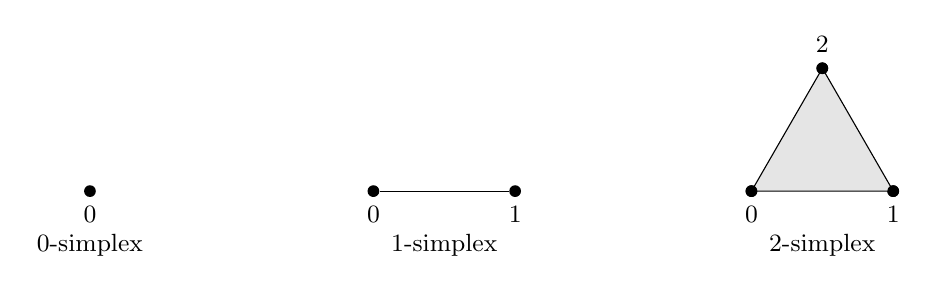
\begin{tikzpicture}[scale=1.2, every node/.style={font=\small}]

% ---- 0-simplex ----
\node[circle, fill=black, inner sep=1.5pt] (v0) at (0,0) {};
\node[below=2pt] at (v0) {$0$};
\node[below=12pt] at (0,0) {0-simplex};

% ---- 1-simplex ----
\node[circle, fill=black, inner sep=1.5pt] (v1a) at (3,0) {};
\node[circle, fill=black, inner sep=1.5pt] (v1b) at (4.5,0) {};

\draw (v1a) -- (v1b);

\node[below=2pt] at (v1a) {$0$};
\node[below=2pt] at (v1b) {$1$};

\node[below=12pt] at (3.75,0) {1-simplex};

% ---- 2-simplex ----
\node[circle, fill=black, inner sep=1.5pt] (v2a) at (7,0) {};
\node[circle, fill=black, inner sep=1.5pt] (v2b) at (8.5,0) {};
\node[circle, fill=black, inner sep=1.5pt] (v2c) at (7.75,1.3) {};

% \filldraw[fill=gray!20, draw=black] 
%   (v2a.center) -- (v2b.center) -- (v2c.center) -- cycle;
\draw[fill=gray!20] (v2a.center) -- (v2b.center) -- (v2c.center) -- cycle;

\node[circle, fill=black, inner sep=1.5pt] at (v2a.center) {};
\node[circle, fill=black, inner sep=1.5pt] at (v2b.center) {};
\node[circle, fill=black, inner sep=1.5pt] at (v2c.center) {};

\node[below=2pt] at (v2a) {$0$};
\node[below=2pt] at (v2b) {$1$};
\node[above=2pt] at (v2c) {$2$};

\node[below=12pt] at (7.75,0) {2-simplex};

\end{tikzpicture}
$$

For this reason, the zero-simplex is called vertices, the one-simplex edges, and the two-simplex triangles.

The geometric realisation of horns can be visualised as removing certain faces from the standard simplices, which are also demonstrated below.
% Demonstration of horns in 2-simplex
$$
\begin{tikzpicture}[scale=1.2, every node/.style={font=\small}]

% ---- 0-simplex ----
\node[circle, fill=black, inner sep=1.5pt] (v0a) at (0,0) {};
\node[circle, fill=black, inner sep=1.5pt] (v0b) at (1.5,0) {};
\node[circle, fill=black, inner sep=1.5pt] (v0c) at (0.75,1.3) {};
\node[below=2pt] at (v0) {$0$};

\draw (v0b) -- (v0a) -- (v0c);

\node[below=2pt] at (v0a) {$0$};
\node[below=2pt] at (v0b) {$1$};
\node[above=2pt] at (v0c) {$2$};

\node[below=12pt] at (0.75,0) {$|\L^2_0|$};

% ---- 1-simplex ----
\node[circle, fill=black, inner sep=1.5pt] (v1a) at (3.5,0) {};
\node[circle, fill=black, inner sep=1.5pt] (v1b) at (5,0) {};
\node[circle, fill=black, inner sep=1.5pt] (v1c) at (4.25,1.3) {};

\draw (v1a) -- (v1b) -- (v1c);

\node[below=2pt] at (v1a) {$0$};
\node[below=2pt] at (v1b) {$1$};
\node[above=2pt] at (v1c) {$2$};

\node[below=12pt] at (4.25,0) {$|\L^2_1|$};

% ---- 2-simplex ----
\node[circle, fill=black, inner sep=1.5pt] (v2a) at (7,0) {};
\node[circle, fill=black, inner sep=1.5pt] (v2b) at (8.5,0) {};
\node[circle, fill=black, inner sep=1.5pt] (v2c) at (7.75,1.3) {};

% \filldraw[fill=gray!20, draw=black] 
\draw (v2a.center) -- (v2c.center) -- (v2b.center);

\node[below=2pt] at (v2a) {$0$};
\node[below=2pt] at (v2b) {$1$};
\node[above=2pt] at (v2c) {$2$};

\node[below=12pt] at (7.75,0) {$|\L^2_2|$};

\end{tikzpicture}
$$


In fact, we have the following theorem.

\begin{theorem}
	The geometric realisation functor $| - |: \sS \to \text{KHaus}$ is equivalent to 
	$$
		|X| = \text{colim}_{\Delta^n \to X} |\Delta^n|
	$$
	where the colimit is considered over the category of compactly generated Hausdorff spaces.
\end{theorem}
